%
% The first command in your LaTeX source must be the \documentclass command.
\documentclass[sigconf]{acmart}

%
% defining the \BibTeX command - from Oren Patashnik's original BibTeX documentation.
\def\BibTeX{{\rm B\kern-.05em{\sc i\kern-.025em b}\kern-.08emT\kern-.1667em\lower.7ex\hbox{E}\kern-.125emX}}
    
% Rights management information. 
% This information is sent to you when you complete the rights form.
% These commands have SAMPLE values in them; it is your responsibility as an author to replace
% the commands and values with those provided to you when you complete the rights form.
%
% These commands are for a PROCEEDINGS abstract or paper.
\copyrightyear{2018}
\acmYear{2018}
\setcopyright{acmlicensed}
\acmConference[Woodstock '18]{Woodstock '18: ACM Symposium on Neural Gaze Detection}{June 03--05, 2018}{Woodstock, NY}
\acmBooktitle{Woodstock '18: ACM Symposium on Neural Gaze Detection, June 03--05, 2018, Woodstock, NY}
\acmPrice{15.00}
\acmDOI{10.1145/1122445.1122456}
\acmISBN{978-1-4503-9999-9/18/06}

%
% These commands are for a JOURNAL article.
%\setcopyright{acmcopyright}
%\acmJournal{TOG}
%\acmYear{2018}\acmVolume{37}\acmNumber{4}\acmArticle{111}\acmMonth{8}
%\acmDOI{10.1145/1122445.1122456}

%
% Submission ID. 
% Use this when submitting an article to a sponsored event. You'll receive a unique submission ID from the organizers
% of the event, and this ID should be used as the parameter to this command.
%\acmSubmissionID{123-A56-BU3}

%
% The majority of ACM publications use numbered citations and references. If you are preparing content for an event
% sponsored by ACM SIGGRAPH, you must use the "author year" style of citations and references. Uncommenting
% the next command will enable that style.
%\citestyle{acmauthoryear}

%
% end of the preamble, start of the body of the document source.
\begin{document}

%
% The "title" command has an optional parameter, allowing the author to define a "short title" to be used in page headers.
\title{Grand Challenge: A Real-Time Multi-label Classifier for High-Speed Streaming Data}

%
% The "author" command and its associated commands are used to define the authors and their affiliations.
% Of note is the shared affiliation of the first two authors, and the "authornote" and "authornotemark" commands
% used to denote shared contribution to the research.


\author{Kia Teymourian}
\affiliation{%
  \institution{Boston University}
 }
\email{kiat@bu.edu}

\author{Sambasiva Rao Gangineni}
\affiliation{%
  \institution{Boston University}  
}
\email{samba693@bu.edu}

\author{Harshad Reddy Nalla}
\affiliation{%
	\institution{Boston University}  
}
\email{harshad@bu.edu}

\author{Dimitrije Jankov}
\affiliation{%
	\institution{Rice University}  
}
\email{dimitrijejankov@gmail.com}

\author{Saeed Fathollahzadeh}
\affiliation{%
	\institution{Iran University of Science and Technology}  
}
\email{fathollahzadeh@comp.iust.ac.ir}



%
% By default, the full list of authors will be used in the page headers. Often, this list is too long, and will overlap
% other information printed in the page headers. This command allows the author to define a more concise list
% of authors' names for this purpose.
\renewcommand{\shortauthors}{Kia Teymourian, et al.}

%
% The abstract is a short summary of the work to be presented in the article.
\begin{abstract}
The winners of the challenge are announced during the conference. The 2019 DEBS Grand Challenge focuses on the application of machine learning to LiDAR data. The goal of the challenge is to perform classification of objects in different scenes surveyed by the LiDAR. The applications of LIDAR and object detection go well beyond autonomous vehicles and are suitable for use in agriculture, waterway maintenance and flood prevention, and construction.

In this paper, we describe our implementation for ACM DEBS 2019 Grand Challenge for a high-speed online neural network classifier that is highly customized to classify objects from streaming data in real-time.
\end{abstract}

%
% The code below is generated by the tool at http://dl.acm.org/ccs.cfm.
% Please copy and paste the code instead of the example below.
%
\begin{CCSXML}
<ccs2012>
 <concept>
  <concept_id>10010520.10010553.10010562</concept_id>
  <concept_desc>Computer systems organization~Embedded systems</concept_desc>
  <concept_significance>500</concept_significance>
 </concept>
 <concept>
  <concept_id>10010520.10010575.10010755</concept_id>
  <concept_desc>Computer systems organization~Redundancy</concept_desc>
  <concept_significance>300</concept_significance>
 </concept>
 <concept>
  <concept_id>10010520.10010553.10010554</concept_id>
  <concept_desc>Computer systems organization~Robotics</concept_desc>
  <concept_significance>100</concept_significance>
 </concept>
 <concept>
  <concept_id>10003033.10003083.10003095</concept_id>
  <concept_desc>Networks~Network reliability</concept_desc>
  <concept_significance>100</concept_significance>
 </concept>
</ccs2012>
\end{CCSXML}

\ccsdesc[500]{Information Systems~Machine Learning}
\ccsdesc[300]{Information Systems~Data Stream}

%
% Keywords. The author(s) should pick words that accurately describe the work being
% presented. Separate the keywords with commas.
\keywords{neural networks, multi-label classification, data stream processing}



%
% This command processes the author and affiliation and title information and builds
% the first part of the formatted document.
\maketitle

\section{Introduction}
Many real-world applications include multi-lable data and require real-time high-speed multi-lable classification. In most application, it is crucial to proactively react based on classification results. For example, in autonomous car application it is important to detect surrounding cars and pedestrians in real-time to send reaction signals. 

\section{Data Set}
DEBS 2019  Challenge provides a training and test data sets \cite{DEBSGC2019}. 
The data set consist of LiDAR sensor point cloud which has 64 lasers. Each scene includes 72,000 data readings which includes  X, Y, and Z coordinates (Y axis is the shown to be the elevation). 
In each scene objects are placed around the LiDAR scanner and data is collected, example objects are \textbf{ATM machine}, \textbf{pedestrian}, \textbf{benches}, \textbf{cloth recycling container}. 

We build multiple 2D and 3D visualizations of the data like shown in Figures \ref{fig:ground_before},  \ref{fig:after} and \ref{fig:ClusteringWithNoiseFiltering}. 
We also created animated images of the sequences of scenes to see if the sequence of scenes have any relations to each other. 
We observed that sequence of scenes have no relations and scenes are randomly selected from a set of scenes. 
However, in applications like autonomous vehicles, sequences of scenes have a correlations so 
that one can track the object coming in range of LiDAR laser and going out of the range. 
This information could be used to improved the classification accuracy such application.    


% SAEED
% The data provided for the challenge consists of point cloud readings simulated for a LiDAR sensor that mounts 64 lasers Fig.\ref{fig:data_overview} a , each shoot 1125 times per rotation. That is, each scene consists of 72,000 readings. Each reading is composed of attributes where X, Y, and Z coordinates are as presented in Fig.\ref{fig:data_overview} b.
% 
% In each scene, objects are representative of urban environments and are of the following types: \textbf{ATM machine}, \textbf{pedestrian}, \textbf{benches}, \textbf{cloth recycling container}, \textbf{drinking fountain}, \textbf{electrical cabinet}, \textbf{emergency phone}, \textbf{fire hydrant}, \textbf{glass recycling container}, \textbf{ice freeze container}, \textbf{mailbox}, \textbf{trash bins}, \textbf{phone booth}, \textbf{trees}, and \textbf{several vehicle types}. In some cases, it is possible for an object in a scene to be hidden from the LiDAR sensor (e.g., when such object is occluded by other objects in the scene)\cite{DEBSGC2019}.


% 
% \begin{figure*}[!ht]
% \begin{center}
%   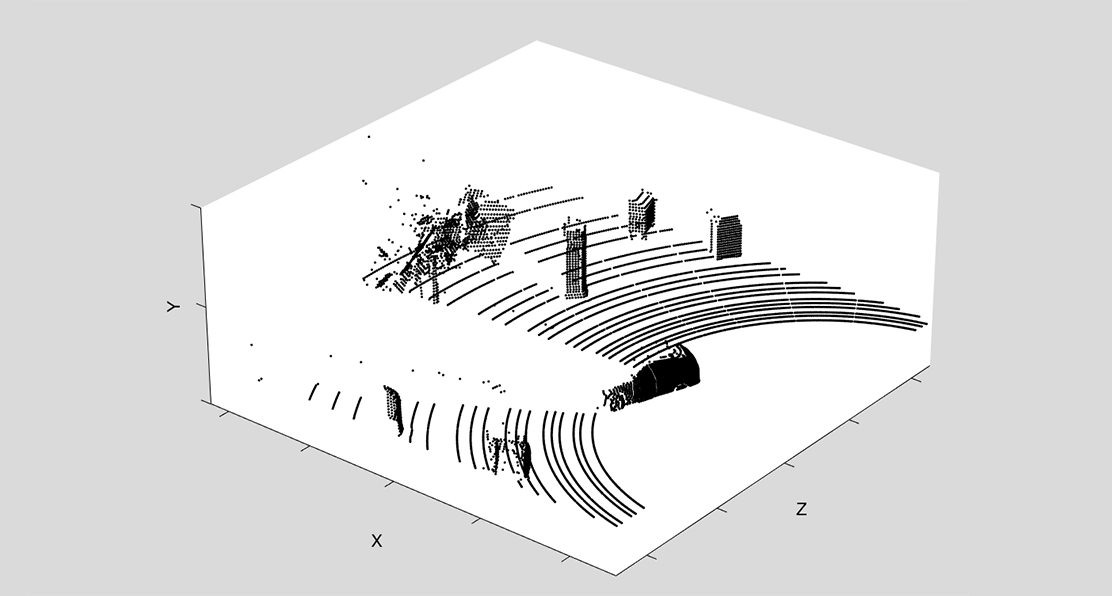
\includegraphics[width=0.8\textwidth]{./images/GC1.png}
%   \caption{An Overview of Data Set from Point Cloud of a single Scene}
%   \label{fig:data_overview}
% \end{center}
% \end{figure*}

%\usepackage{graphics} is needed for \includegraphics


% \begin{figure}%
% 	\centering
% 	\subfloat[point cloud readings simulated for a LiDAR sensor]{{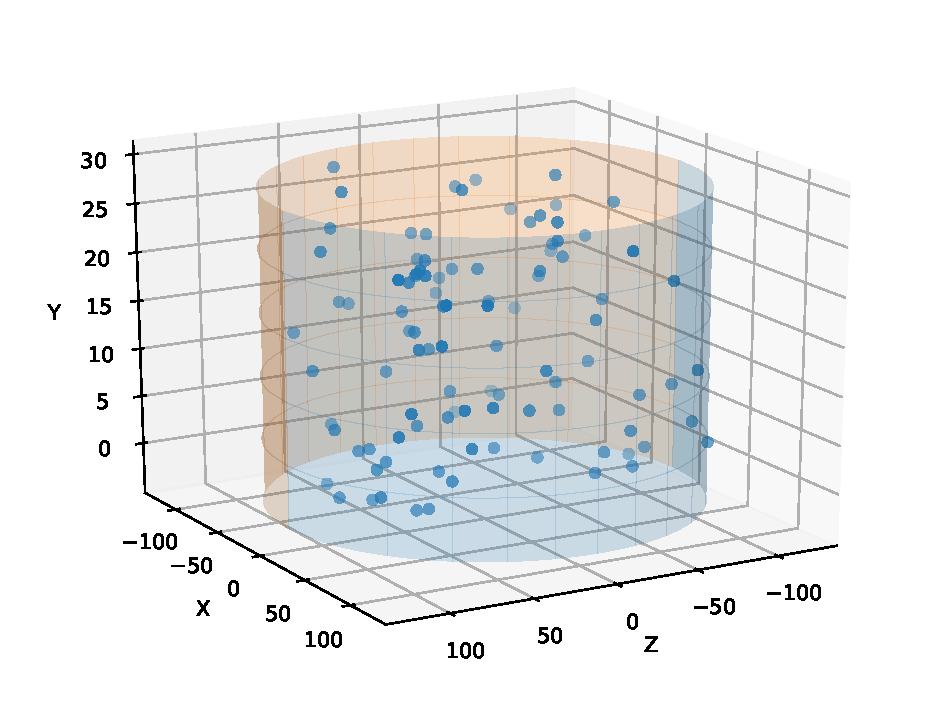
\includegraphics[width=7cm]{images/data_overview.pdf} }}%
% 	\qquad
% 	\subfloat[a scene with different numbers of objects]{{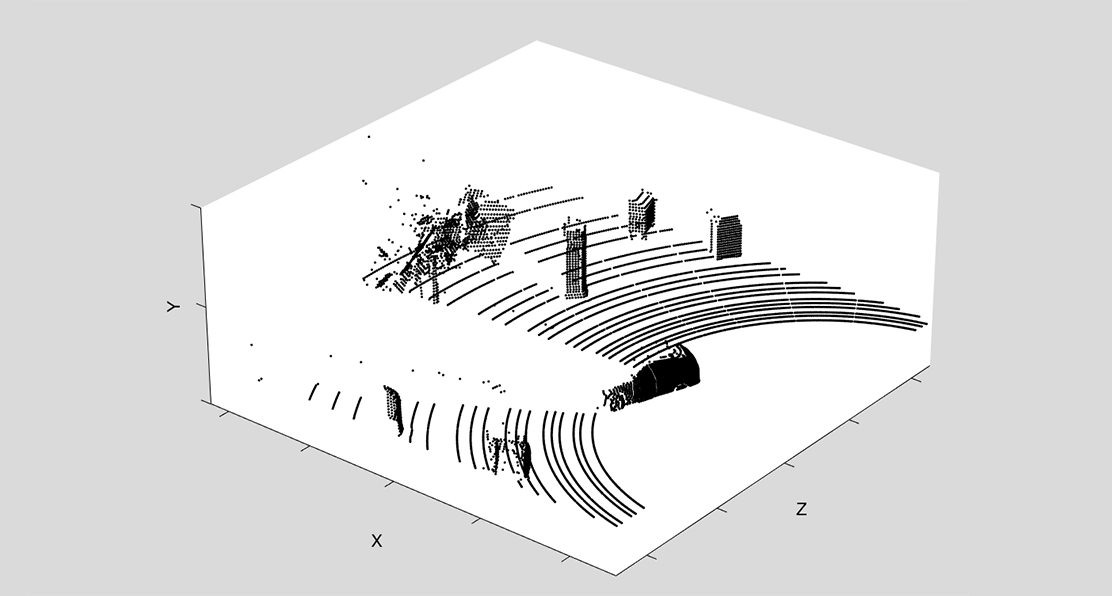
\includegraphics[width=5cm]{images/GC1.png} }}%
% 	\caption{An Overview of Data Set from Point Cloud of a single Scene}%
% 	\label{fig:data_overview}%
% \end{figure}


%KIA 
%Briefly describe the data set and cite the main grand challange paper. 

%We just need to describe what the data is about. 

% We need to mention other data sets like The KITTI Dataset \cite{Geiger2013IJRR}


% KITTI Dataset \cite{Geiger2013IJRR}
\section{Architecture}\label{sec:Architecture}




% Describe the data processing pipeline here. 


% 1. Get the raw data and remove the ground (LiDAR data clean up)
% 2. Segment data and sent it to classifier 
% 3. Classification with Neural Network. 


Figure \ref{fig:dataPipeline} depicts  

\begin{figure*}[h!]
 \begin{center}
   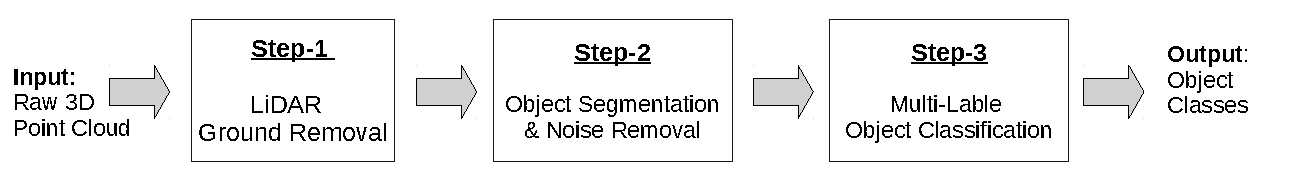
\includegraphics[width=0.9\textwidth]{./images/DataProcessingPipleline.pdf}
   \caption{An Overview of our Data Processing Architecture}
   \label{fig:dataPipeline}
 \end{center}
\end{figure*}





Describe \ldots. 

Different forms of data processing architectures that we have implemented and tested . 

\begin{enumerate}
  \item Different methods for removing noise from raw data (data preprocessing). 
  \item Projecting 3D data into 2D data using 3 different projection methods 
  \item CNN  (with and without maxpool) + fully-connected + dropout + fully-connected+softmax
  \item CNN with different number of hidden layers. 

\end{enumerate}



% KIA
% We need another image to describe the CNN architecture. 
% Add two images about it. 




\section{Conclusion and Future Work}\label{sec:conclusion}











\section{Evaluation}\label{sec:Evaluation}

\TODO{Describe the evaluation set up briefly.}



\TODO{- 3 Graph that compares the prcision/recall (F1) and time perofrmance of our multiple approaches. 
}


\TODO{Our appriaches are: 
1. Graphs for 2D CNN with simple linear projection on one of the axis.
2. 2D CNN with improved transformation from 3D to 2D CNN
3. 2D CNN - with - separation and projection and then segmentation with DBSCAN 
4. 3D CNN
5. Different No. of Layers up to 3 and 2 different size of filter. 
 }


- We should run it on a standard machine (better on EC2 because it is better reproducable) and show the processong time performance. 


- We present on our plots, Precision/Recall and Processing time. 







\bibliographystyle{ACM-Reference-Format}
\bibliography{refrences}




\end{document}
